\documentclass{beamer}

\pdfmapfile{+sansmathaccent.map}


\mode<presentation>
{
	\usetheme{Warsaw} % or try Darmstadt, Madrid, Warsaw, Rochester, CambridgeUS, ...
	\usecolortheme{seahorse} % or try seahorse, beaver, crane, wolverine, ...
	\usefonttheme{serif}  % or try serif, structurebold, ...
	\setbeamertemplate{navigation symbols}{}
	\setbeamertemplate{caption}[numbered]
} 


%%%%%%%%%%%%%%%%%%%%%%%%%%%%
% itemize settings

\definecolor{myhotpink}{RGB}{255, 80, 200}
\definecolor{mywarmpink}{RGB}{255, 60, 160}
\definecolor{mylightpink}{RGB}{255, 80, 200}
\definecolor{mypink}{RGB}{255, 30, 80}
\definecolor{mydarkpink}{RGB}{155, 25, 60}

\definecolor{mypaleblue}{RGB}{240, 240, 255}
\definecolor{mylightblue}{RGB}{120, 150, 255}
\definecolor{myblue}{RGB}{90, 90, 255}
\definecolor{mygblue}{RGB}{70, 110, 240}
\definecolor{mydarkblue}{RGB}{0, 0, 180}
\definecolor{myblackblue}{RGB}{40, 40, 120}

\definecolor{mygreen}{RGB}{0, 200, 0}
\definecolor{mygreen2}{RGB}{245, 255, 230}

\definecolor{mygray}{gray}{0.8}
\definecolor{mydarkgray}{RGB}{80, 80, 160}

\definecolor{mydarkred}{RGB}{160, 30, 30}
\definecolor{mylightred}{RGB}{255, 150, 150}
\definecolor{myred}{RGB}{200, 110, 110}
\definecolor{myblackred}{RGB}{120, 40, 40}

\definecolor{mygreen}{RGB}{0, 200, 0}
\definecolor{mygreen2}{RGB}{205, 255, 200}

\definecolor{mydarkcolor}{RGB}{60, 25, 155}
\definecolor{mylightcolor}{RGB}{130, 180, 250}

\setbeamertemplate{itemize items}[default]

\setbeamertemplate{itemize item}{\color{myblackblue}$\blacksquare$}
\setbeamertemplate{itemize subitem}{\color{mydarkblue}$\blacktriangleright$}
\setbeamertemplate{itemize subsubitem}{\color{mygray}$\blacksquare$}

\setbeamercolor{palette quaternary}{fg=white,bg=mygblue} %mydarkgray
\setbeamercolor{titlelike}{parent=palette quaternary}

\setbeamercolor{palette quaternary2}{fg=white,bg=mygblue}%black myblue
\setbeamercolor{frametitle}{parent=palette quaternary2}

\setbeamerfont{frametitle}{size=\Large,series=\scshape}
\setbeamerfont{framesubtitle}{size=\normalsize,series=\upshape}


%%%%%%%%%%%%%%%%%%%%%%%%%%%%
% block settings

%\setbeamercolor{block title}{bg=red!50,fg=black}
%\setbeamercolor{block title}{bg=mylightblue,fg=black}
\setbeamercolor{block title}{bg=myblackblue,fg=white}

\setbeamercolor*{block title example}{bg=mygreen!40!white,fg=black}

\setbeamercolor*{block body example}{fg= black,
	bg= mygreen2}


%%%%%%%%%%%%%%%%%%%%%%%%%%%%
% URL settings
\hypersetup{
	colorlinks=false,
	linkcolor=blue,
	filecolor=blue,      
	urlcolor=blue,
}

%%%%%%%%%%%%%%%%%%%%%%%%%%

\renewcommand{\familydefault}{\rmdefault}

\usepackage{amsmath}
\usepackage{mathtools}

\usepackage{subcaption}

\usepackage{qrcode}

\DeclareMathOperator*{\argmin}{arg\,min}
\newcommand{\bo}[1] {\mathbf{#1}}

\newcommand{\dx}[1] {\dot{\mathbf{#1}}}
\newcommand{\ma}[4] {\begin{bmatrix}
		#1 & #2 \\ #3 & #4
\end{bmatrix}}
\newcommand{\myvec}[2] {\begin{bmatrix}
		#1 \\ #2
\end{bmatrix}}
\newcommand{\myvecT}[2] {\begin{bmatrix}
		#1 & #2
\end{bmatrix}}

\newcommand{\R}{\mathbb{R}} 
\newcommand{\T}{^\top}     



\newcommand{\mydate}{Spring 2023}

\newcommand{\mygit}{\textcolor{blue}{\href{https://github.com/SergeiSa/Computational-Intelligence-Slides-Spring-2023}{github.com/SergeiSa/Computational-Intelligence-Slides-Spring-2023}}}

\newcommand{\myqr}{ \textcolor{black}{\qrcode[height=1.5in]{https://github.com/SergeiSa/Computational-Intelligence-Slides-Spring-2023}}
}

\newcommand{\myqrframe}{
	\begin{frame}
		\centerline{Lecture slides are available via Github, links are on Moodle}
		\bigskip
		\centerline{You can help improve these slides at:}
		\centerline{\mygit}
		\bigskip
		\myqr
	\end{frame}
}


\newcommand{\bref}[2] {\textcolor{blue}{\href{#1}{#2}}}



%%%%%%%%%%%%%%%%%%%%%%%%%%%%
% code settings

\usepackage{listings}
\usepackage{color}
% \definecolor{mygreen}{rgb}{0,0.6,0}
% \definecolor{mygray}{rgb}{0.5,0.5,0.5}
\definecolor{mymauve}{rgb}{0.58,0,0.82}
\lstset{ 
	backgroundcolor=\color{white},   % choose the background color; you must add \usepackage{color} or \usepackage{xcolor}; should come as last argument
	basicstyle=\footnotesize,        % the size of the fonts that are used for the code
	breakatwhitespace=false,         % sets if automatic breaks should only happen at whitespace
	breaklines=true,                 % sets automatic line breaking
	captionpos=b,                    % sets the caption-position to bottom
	commentstyle=\color{mygreen},    % comment style
	deletekeywords={...},            % if you want to delete keywords from the given language
	escapeinside={\%*}{*)},          % if you want to add LaTeX within your code
	extendedchars=true,              % lets you use non-ASCII characters; for 8-bits encodings only, does not work with UTF-8
	firstnumber=0000,                % start line enumeration with line 0000
	frame=single,	                   % adds a frame around the code
	keepspaces=true,                 % keeps spaces in text, useful for keeping indentation of code (possibly needs columns=flexible)
	keywordstyle=\color{blue},       % keyword style
	language=Octave,                 % the language of the code
	morekeywords={*,...},            % if you want to add more keywords to the set
	numbers=left,                    % where to put the line-numbers; possible values are (none, left, right)
	numbersep=5pt,                   % how far the line-numbers are from the code
	numberstyle=\tiny\color{mygray}, % the style that is used for the line-numbers
	rulecolor=\color{black},         % if not set, the frame-color may be changed on line-breaks within not-black text (e.g. comments (green here))
	showspaces=false,                % show spaces everywhere adding particular underscores; it overrides 'showstringspaces'
	showstringspaces=false,          % underline spaces within strings only
	showtabs=false,                  % show tabs within strings adding particular underscores
	stepnumber=2,                    % the step between two line-numbers. If it's 1, each line will be numbered
	stringstyle=\color{mymauve},     % string literal style
	tabsize=2,	                   % sets default tabsize to 2 spaces
	title=\lstname                   % show the filename of files included with \lstinputlisting; also try caption instead of title
}

%%%%%%%%%%%%%%%%%%%%%%%%%%%%
% tikz settings

\usepackage{tikz}
\tikzset{every picture/.style={line width=0.75pt}}

%%%%%%%%%%%%%%%%%%%%%%%%%%%%




\title{Quadratic programming}
\subtitle{Computational Intelligence, Lecture 7}
\author{by Sergei Savin}
\centering
\date{\mydate}



\begin{document}
\maketitle


\begin{frame}{Content}

\begin{itemize}
\item  Quadratic programming
\item  Quadratically constrained quadratic programming (QCQP)
	\begin{itemize}
		\item  QCQP to LP; QCQP to LP
		\item  Ellipsoidal constraints $\rightarrow$ to canonical form
	\end{itemize}
\end{itemize}

\end{frame}




\begin{frame}{Positive-definite matrices}
	%\framesubtitle{General form}
	\begin{flushleft}
		
		Positive-definite matrices the following properties:
		
		\begin{block}{Eigenvalues}
			All eigenvalues of a positive-definite (PD) matrix are real and positive.
		\end{block}
	
		\begin{block}{Eigenvectors}
			Eigenvectors of a PD matrix with form an orthogonal basis.
		\end{block}
	
		Proof (for the case of distinct eigenvalues): let $\bo{M}$ be a PD matrix, and $\bo{M}\bo{v} = \lambda \bo{v}$ and  $\bo{M}\bo{u} = \gamma \bo{u}$. Then:
		%
		\begin{align}
			\bo{u}\T\bo{M}\bo{v} = \bo{u}\T(\bo{M}\bo{v})= \lambda \bo{u}\T \bo{v} \\
			\bo{u}\T\bo{M}\bo{v} = (\bo{u}\T\bo{M})\bo{v}= \gamma \bo{u}\T \bo{v}
		\end{align}
		
		Therefore, $ \lambda \bo{u}\T \bo{v}= \gamma \bo{u}\T \bo{v}$, and since $\lambda$ and $ \gamma$ are eigenvalues and and eigenvalues are distinct, so $\lambda \neq \gamma$. This implies that $\bo{u}\T \bo{v} = 0$.
		
	\end{flushleft}
\end{frame}




\begin{frame}{Quadratic programming}
%\framesubtitle{General form}
\begin{flushleft}

Remember the general form of a quadratic program:

%
\begin{equation}
	\begin{aligned}
		& \underset{\bo{x}}{\text{minimize}}
		& & \bo{x}^\top \bo{H} \bo{x} + \bo{f}^\top\bo{x}, \\
		& \text{subject to}
		& & \begin{cases}
			\bo{A}\bo{x} \leq \bo{b}, \\
			\bo{F}\bo{x} = \bo{g}.
		\end{cases}
	\end{aligned}
\end{equation}

where $\bo{H}$ is positive-definite and $\bo{A}\bo{x} \leq \bo{b}$ describe a convex region.
 
\end{flushleft}
\end{frame}



\begin{frame}{Geometry of a QP}
	%\framesubtitle{General form}
	\begin{flushleft}
		
		% TODO: \usepackage{graphicx} required
		\begin{figure}
			\centering
			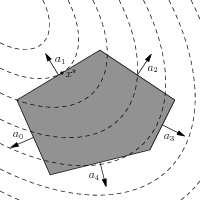
\includegraphics[width=0.5\linewidth]{qpcontour}
			\caption{Geometry of a QP. \bref{https://docs.mosek.com/modeling-cookbook/qcqo.html}{Source}}
			\label{fig:qpcontour}
		\end{figure}
		
		
	\end{flushleft}
\end{frame}





\begin{frame}{Cost function of a QP, 1}
	%\framesubtitle{General form}
	\begin{flushleft}
		
		The cost function of a QP has the form $c(\bo{x}) = \bo{x}^\top \bo{H} \bo{x} + \bo{f}^\top\bo{x}$. Let us show that the requirement that $\mathbf{H}$ is positive-definite does not limit the range of convex problems that can be solved as a QP.
		
		\bigskip
		
		Let $\bo{M}$ be a non-symmetric matrix. Quadratic form $q(\bo{x}) = \bo{x}\T \bo{M} \bo{x}$ is a scalar and is equal to its transpose:
		%
		\begin{align}
			q(\bo{x}) = \bo{x}\T \bo{M} \bo{x} \\
			q(\bo{x}) = 0.5 (\bo{x}\T \bo{M} \bo{x} + \bo{x}\T \bo{M} \bo{x}) \\
			q(\bo{x}) = 0.5 (\bo{x}\T \bo{M} \bo{x} + \bo{x}\T \bo{M}\T \bo{x}) \\
			q(\bo{x}) = 0.5 \bo{x}\T( \bo{M} + \bo{M}\T )\bo{x}
		\end{align}
	
		Equivalently prove that the cost function $c(\bo{x})$ is always equivalent to the cost function $c(\bo{x}) = 0.5 \bo{x}^\top (\bo{H} + \bo{H}\T) \bo{x} + \bo{f}^\top\bo{x}$. Because of that, without a loss of generality we can assume $\bo{H}$ to be symmetric.
		
	\end{flushleft}
\end{frame}


\begin{frame}{Cost function of a QP, 2}
	%\framesubtitle{General form}
	\begin{flushleft}
		
		Let us prove that $\bo{H}$ needs to be positive semi-definite in order for $c(\bo{x})$ to be convex.
		
		\bigskip
		
		Assume that one of the eigenvalues of $\bo{H}$ is negative: $\bo{H}\bo{v} = \lambda\bo{v}$, where $\lambda < 0$ and $||\bo{v}|| = 1$. We can find values of $c(0)$, $c(\bo{v})$ and $c(2\bo{v})$:
		%
		\begin{align}
			c(0) &= 0 \\
			c(\bo{v}) &= \bo{v}\T \bo{H}\bo{v} =  \lambda \bo{v}\T \bo{v} =  \lambda
		\end{align}
		
		Note that $c((1 - \beta) 0 + \beta \bo{v}) = c(\beta\bo{v}) =  \lambda \beta^2$ and $(1 - \beta) c(0) + \beta c(\bo{v}) = \lambda \beta$. Since $0 < \beta < 1$ we conclude $\beta^2 < \beta$; since $\lambda < 0$, $\lambda \beta^2 > \lambda \beta$. So $c((1 - \beta) 0 + \beta \bo{v}) >  (1 - \beta) c(0) + \beta c(\bo{v})$. Thus, such $c(\bo{x})$ is not convex. \qed
		
	\end{flushleft}
\end{frame}




\begin{frame}{Degenerate QP}
	%\framesubtitle{General form}
	\begin{flushleft}
		
		Let us consider a QP with degenerate matrix $\bo{H} = \bo{R} \Sigma \bo{R}\T$ (without a loss of generality $\bo{H}$ can be assumed to be symmetric), where $\bo{R} \in \R^{n \times k}$.
		%
		\begin{equation}
			\begin{aligned}
				& \underset{\bo{x}}{\text{minimize}}
				& & \bo{x}^\top \bo{R} \Sigma \bo{R}\T \bo{x} + \bo{f}\T\bo{x}, \\
				& \text{subject to}
				& & \begin{cases}
					\bo{A}\bo{x} \leq \bo{b}, \\
					\bo{F}\bo{x} = \bo{g}.
				\end{cases}
			\end{aligned}
		\end{equation}
		%
		Matrix $\bo{R}$ is a row-space basis of $\bo{H}$, and $\bo{N}$ is its orthogonal compliment. Then we can decompose $\bo{x}$ as $\bo{x} = \bo{R}\zeta+\bo{N}\bo{z}$:
		%
		\begin{equation}
			\begin{aligned}
				& \underset{\zeta, \bo{z}}{\text{minimize}}
				& & \zeta\T \Sigma \zeta + \bo{f}\T\bo{R}\zeta+\bo{f}\T\bo{N}\bo{z}, \\
				& \text{subject to}
				& & \begin{cases}
					\bo{A}\bo{R}\zeta+\bo{A}\bo{N}\bo{z} \leq \bo{b}, \\
					\bo{F}\bo{R}\zeta+\bo{F}\bo{N}\bo{z} = \bo{g}.
				\end{cases}
			\end{aligned}
		\end{equation}
		
	\end{flushleft}
\end{frame}








\begin{frame}{Quadratically constrained quadratic programming}
%\framesubtitle{General form}
\begin{flushleft}

General form of a quadratically constrained quadratic program (QCQP) is given below:

%
\begin{equation}
\begin{aligned}
& \underset{\mathbf{x}}{\text{minimize}}
& & \mathbf{x}^\top \mathbf{P}_0 \mathbf{x} + \mathbf{q}_0^\top\mathbf{x}, \\
& \text{subject to}
& & \begin{cases}
    \mathbf{x}^\top \mathbf{P}_i \mathbf{x} + \mathbf{q}_i^\top\mathbf{x} + r_i \leq 0, \\
    \mathbf{F}\mathbf{x} = \mathbf{g}.
    \end{cases}
\end{aligned}
\end{equation}

where $\mathbf{P}_i$ are positive-definite.
 
\end{flushleft}
\end{frame}



\begin{frame}{QCQP - Domain}
%\framesubtitle{Domain}
\begin{flushleft}

Domain of a QCQP without equality constraints and with no degenerate inequality constraints is an intersection of ellipses:

\begin{figure} [h!]
\begin{center}

\tikzset{every picture/.style={line width=0.75pt}} %set default line width to 0.75pt        

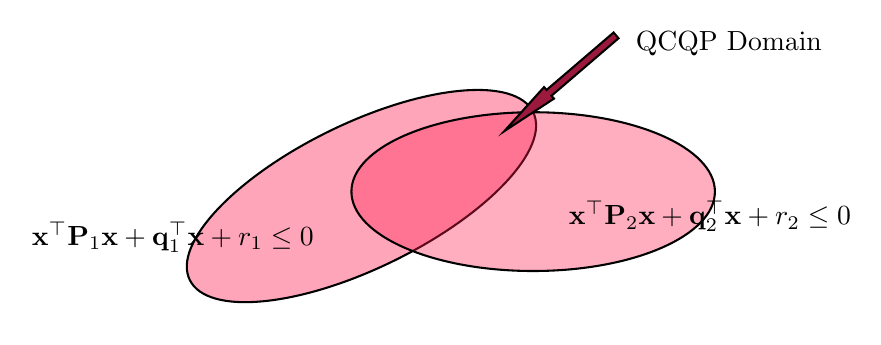
\begin{tikzpicture}[x=0.75pt,y=0.75pt,yscale=-0.75,xscale=0.75]
%uncomment if require: \path (0,300); %set diagram left start at 0, and has height of 300

%Shape: Ellipse [id:dp9898126968799086] 
\draw  [fill=mypink  ,fill opacity=0.4 ] (103.44,199.35) .. controls (92.18,176.27) and (132.43,133.45) .. (193.35,103.71) .. controls (254.27,73.97) and (312.79,68.57) .. (324.06,91.65) .. controls (335.32,114.73) and (295.07,157.55) .. (234.15,187.29) .. controls (173.23,217.03) and (114.71,222.43) .. (103.44,199.35) -- cycle ;
%Shape: Ellipse [id:dp5973223095827915] 
\draw  [fill=mypink  ,fill opacity=0.36 ] (207.31,142.65) .. controls (207.31,114.48) and (259.58,91.65) .. (324.06,91.65) .. controls (388.54,91.65) and (440.81,114.48) .. (440.81,142.65) .. controls (440.81,170.82) and (388.54,193.65) .. (324.06,193.65) .. controls (259.58,193.65) and (207.31,170.82) .. (207.31,142.65) -- cycle ;
%Left Arrow [id:dp11071847750004182] 
\draw  [fill=mydarkpink  ,fill opacity=1 ] (305.5,103.83) -- (331.05,75.5) -- (332.64,77.36) -- (375.73,40.44) -- (378.91,44.15) -- (335.82,81.07) -- (337.41,82.92) -- cycle ;

% Text Node
\draw (0,160) node [anchor=north west][inner sep=0.75pt]    {$\mathbf{x}^\top \mathbf{P}_1 \mathbf{x} + \mathbf{q}_1^\top\mathbf{x} + r_1 \leq 0$};
% Text Node
\draw (345,147) node [anchor=north west][inner sep=0.75pt]    {$\mathbf{x}^\top \mathbf{P}_2 \mathbf{x} + \mathbf{q}_2^\top\mathbf{x} + r_2 \leq 0$};
% Text Node
\draw (388,38) node [anchor=north west][inner sep=0.75pt]   [align=left] {QCQP Domain};


\end{tikzpicture}

\end{center} 
% \caption{AR 601 bipedal robot, Innopolis University}
\end{figure}
 
\end{flushleft}
\end{frame}



\begin{frame}{QCQP to QP and LP}
% \framesubtitle{General form}
\begin{flushleft}

Set $\mathbf{P}_i = \mathbf{0}$ and you get a QP.
%
\begin{equation}
\begin{aligned}
& \underset{\mathbf{x}}{\text{minimize}}
& & \mathbf{x}^\top \mathbf{P}_0 \mathbf{x} + \mathbf{q}_0^\top\mathbf{x}, \\
& \text{subject to}
& & \begin{cases}
    \begin{bmatrix} 
    \mathbf{q}_1^\top \\ ... \\ \mathbf{q}_n^\top
    \end{bmatrix} 
    \mathbf{x} \leq
    \begin{bmatrix} 
    -r_1 \\ ... \\ -r_n
    \end{bmatrix} \\
    \mathbf{F}\mathbf{x} = \mathbf{g}.
    \end{cases}
\end{aligned}
\end{equation}

Set $\mathbf{P}_0 = \mathbf{0}$ and you get an LP.

\end{flushleft}
\end{frame}



\begin{frame}{Turning ellipsoid to the canonical form (1)}
	% \framesubtitle{General form}
	\begin{flushleft}
		
		Can we re-write the expression $\mathbf{x}^\top \mathbf{P} \mathbf{x} + \mathbf{q}^\top\mathbf{x} + r \leq 0$ as a canonical form ellipsoid:
		
		\begin{equation}
			\frac{z_1^2}{m_1^2} + \frac{z_2^2}{m_2^2} + ... + 
			\frac{z_n^2}{m_n^2} \leq 1
		\end{equation}
		
		We start by proposing a substitution $\bo{x}_0 = - \frac{1}{2}\bo{P}^{-1}\bo{q}$ and $-d = r - \bo{x}_0\T \bo{P} \bo{x}_0$. We can prove that: $(\bo{x} - \bo{x}_0)\T \bo{P}(\bo{x} - \bo{x}_0) - d =
		\mathbf{x}^\top \mathbf{P} \mathbf{x} + \mathbf{q}^\top\mathbf{x} + r$
		
		\begin{align}
			(\bo{x} - \bo{x}_0)\T \bo{P}(\bo{x} - \bo{x}_0) - d =
			\\
			= \bo{x}\T\bo{P}\bo{x} - 2\bo{x}_0\T\bo{P}\bo{x} + \bo{x}_0\T\bo{P}\bo{x}_0 - d &=
			\\
			= \bo{x}\T\bo{P}\bo{x} + 2\left(\textcolor{mydarkblue}{\frac{1}{2}\bo{P}^{-1}\bo{q}}\right)\T\bo{P}\bo{x} + \bo{x}_0\T\bo{P}\bo{x}_0 + \textcolor{mydarkblue}{r - \bo{x}_0\T \bo{P} \bo{x}_0} &=
			\\
			= \bo{x}\T\bo{P}\bo{x} + \bo{q}\T \bo{x} + r.
		\end{align}
		
	\end{flushleft}
\end{frame}



\begin{frame}{Turning ellipsoid to the canonical form (2)}
	% \framesubtitle{General form}
	\begin{flushleft}
		
		Thus our original expression became:
		%
		\begin{align}
			(\bo{x} - \bo{x}_0)\T \bo{P}(\bo{x} - \bo{x}_0) - d \leq 0
		\end{align}
	%
		We define $\bo{A} = \sqrt{\bo{P}}$ with SVD decomposition $\bo{A} = \bo{U} \Sigma \bo{V}\T$. Defining $\bo{z} = \bo{V}\T (\bo{x} - \bo{x}_0)$ we get:
	%
	\begin{align}
		(\bo{x} - \bo{x}_0)\T \bo{A}\T\bo{A}(\bo{x} - \bo{x}_0) - d \leq 0 
		\\
		(\bo{x} - \bo{x}_0)\T  \bo{V} \Sigma \bo{U}\T  \bo{U} \Sigma \bo{V}\T(\bo{x} - \bo{x}_0) - d \leq 0 
		\\
		(\bo{x} - \bo{x}_0)\T  \bo{V} \Sigma^2 \bo{V}\T(\bo{x} - \bo{x}_0) - d \leq 0
		\\
		\bo{z}\T   \Sigma^2 \bo{z} - d \leq 0
		\\
		\sum z_i^2 \sigma_i^2  \leq d
	\end{align}
%
Defining $1/m_i^2 = \sigma_i^2 / d$ we get:
%
\begin{equation}
	\frac{z_1^2}{m_1^2} + \frac{z_2^2}{m_2^2} + ... + 
	\frac{z_n^2}{m_n^2} \leq 1
\end{equation}
		
	\end{flushleft}
\end{frame}





\begin{frame}{Homework}
% \framesubtitle{Parameter estimation}
\begin{flushleft}

Implement a program that finds right-most point of an intersection of two ellipsoids; visualise the problem and the solution.

\end{flushleft}
\end{frame}



\begin{frame}{Further reading}
	% \framesubtitle{Local coordinates}
	\begin{flushleft}
		
		\begin{itemize}
			\item \bref{https://mitsloan-php.s3.amazonaws.com/wp-faculty/sites/30/2016/12/15032137/Symmetric-Matrices-and-Eigendecomposition.pdf}{Symmetric Matrices and Eigendecomposition. Robert M. Freund, MIT, 2014}.
			
			\item \bref{https://docs.mosek.com/modeling-cookbook/qcqo.html}{MOSEK, QP and QCQP}.
			
			
		\end{itemize}
		
		
	\end{flushleft}
\end{frame}


\myqrframe



\end{document}
